%!TEX root = ../main.tex

\section{Running Case Study}
\label{sec:appendix_case_study}

In this section, we provide a complete running example of \sys to illustrate the tree-based agentic reasoning process described in Section~\ref{sec:tree_based_agentic_reasoning}.

\begin{figure*}[!t]
    \centering 
    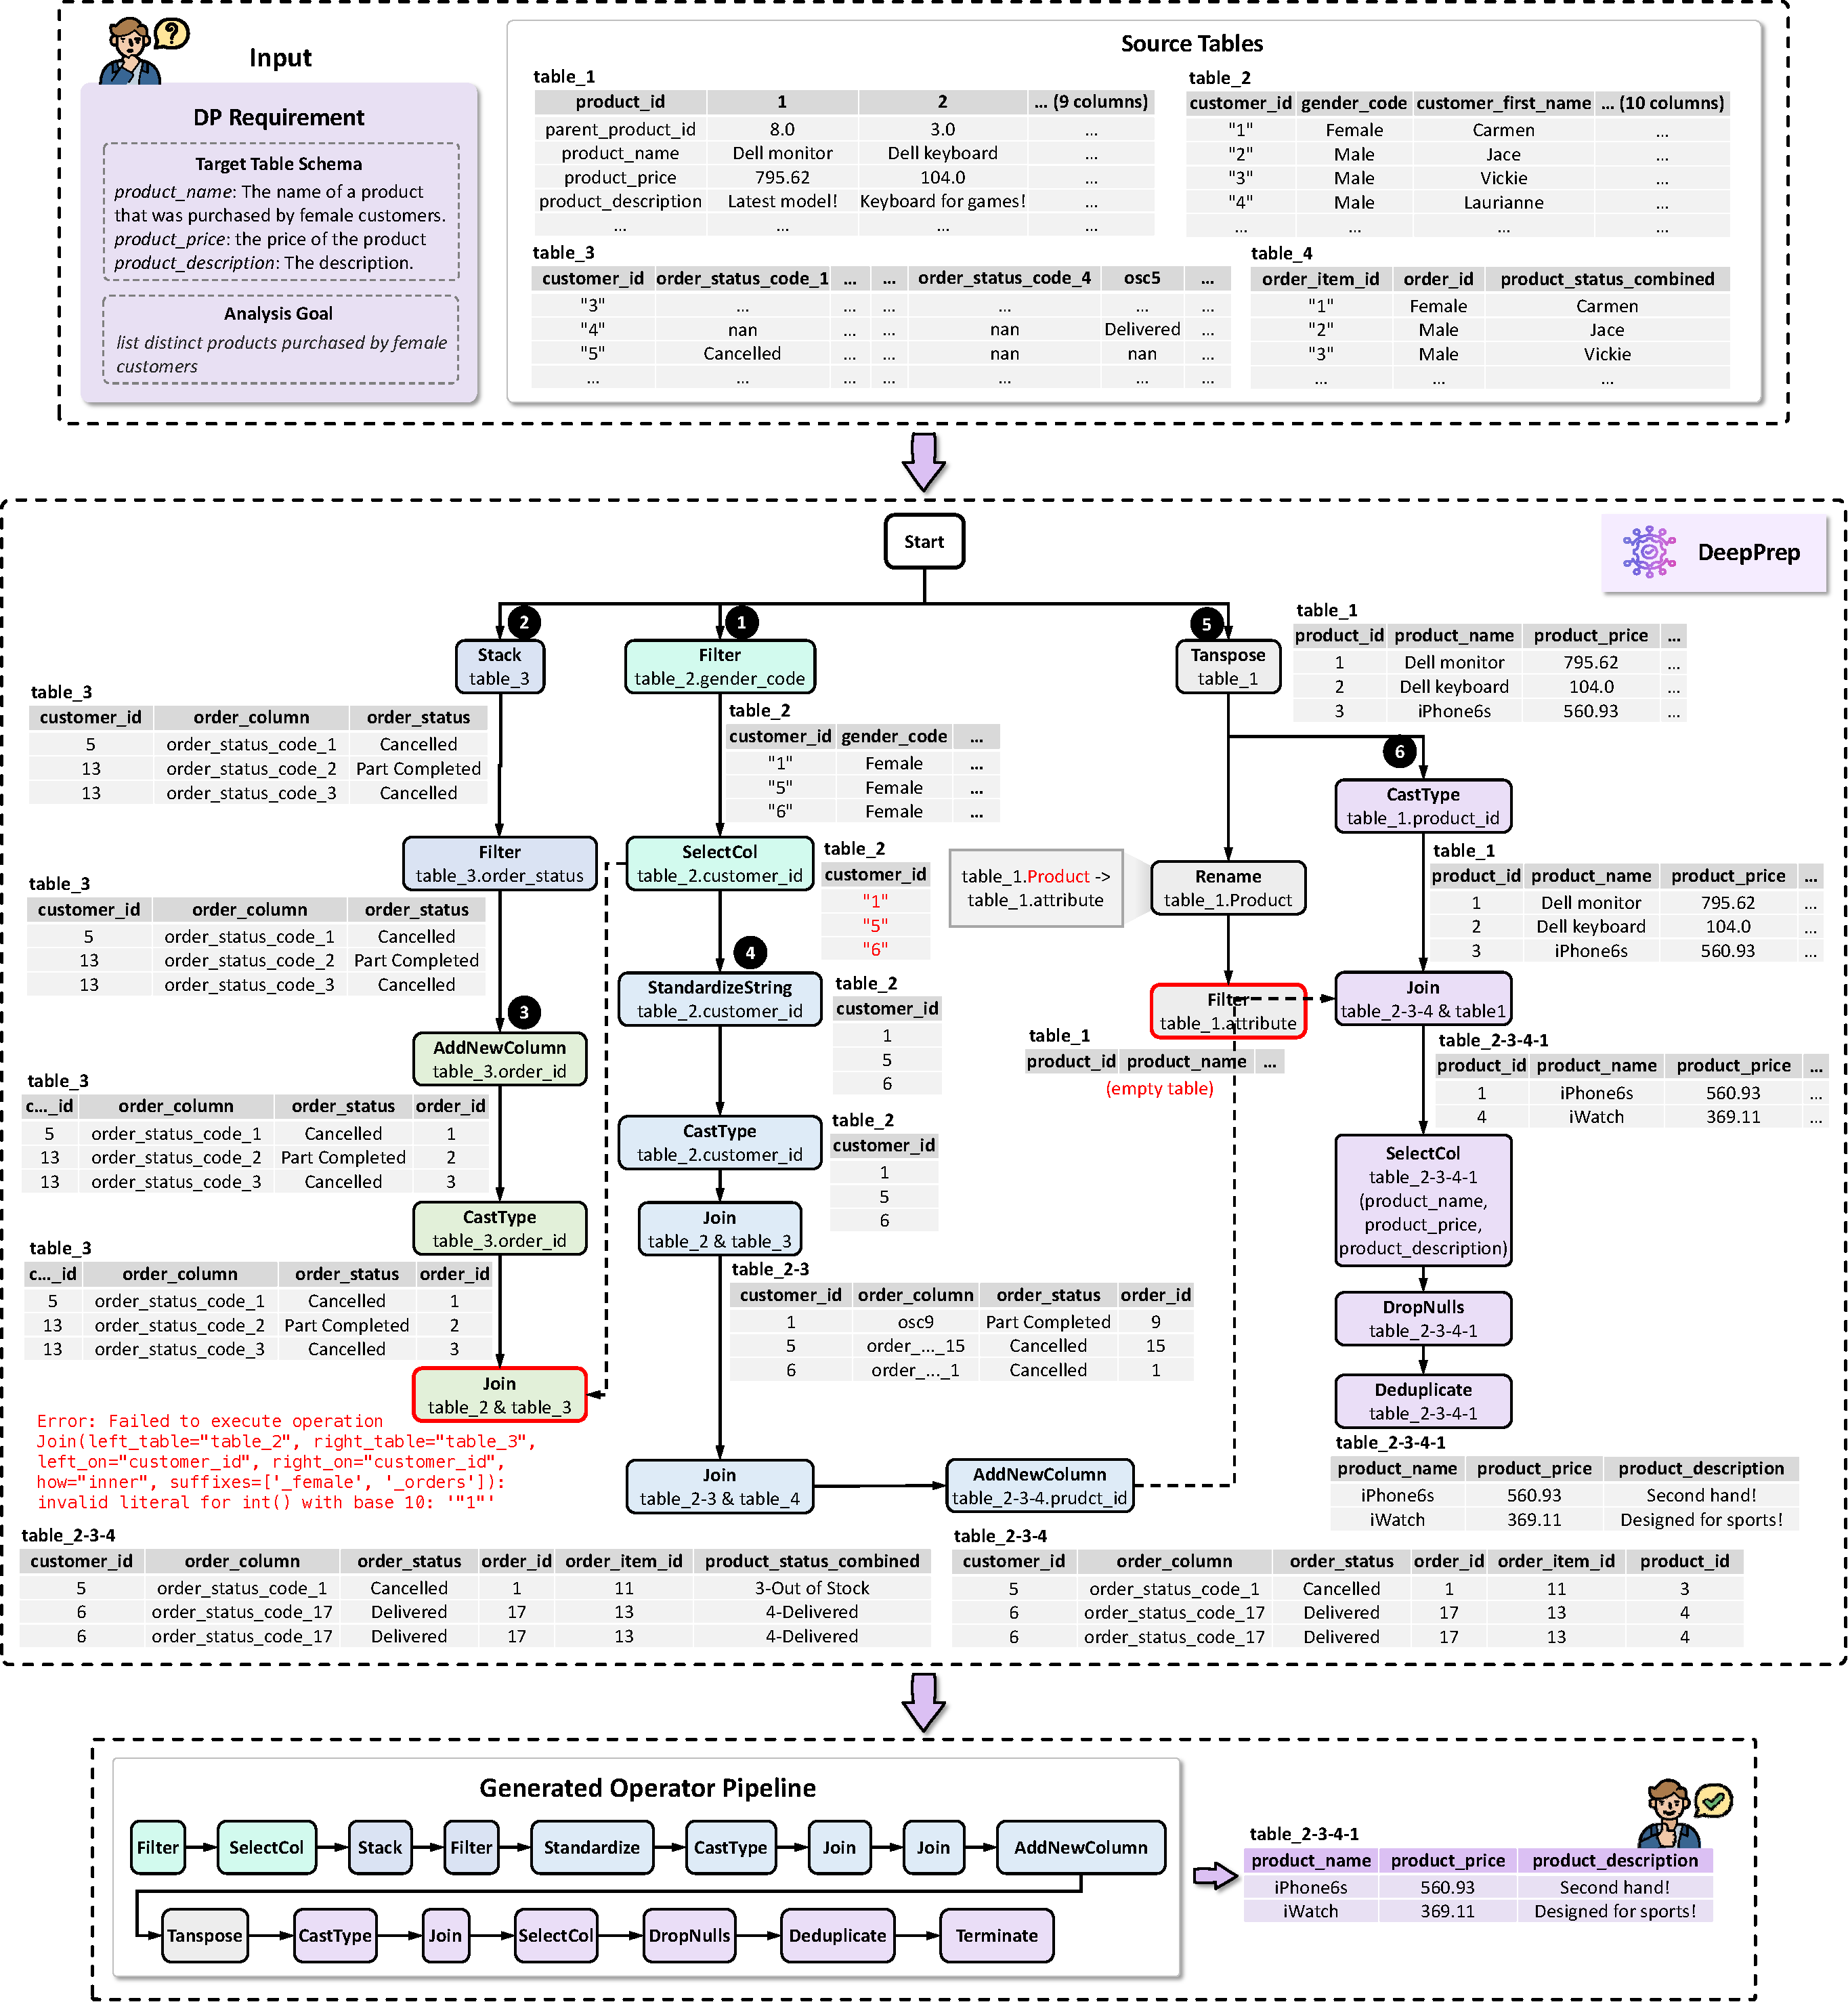
\includegraphics[width=0.99\textwidth]{appendix/figures/fig/case_study.pdf}
    % \vspace{-1em}
    \caption{A real case of \sys. We only show the first 3 rows of intermediate tables due to the space limit.
    }
    \label{fig:case_study}
    % \vspace{-1em}
\end{figure*}


Figure~\ref{fig:case_study} shows a real case of \sys on a data preparation task. Given source tables containing movie, rating, and director information, the goal is to produce a target table with specific columns including movie title, genre, rating, and director name.

\stitle{Step 1: Initial Planning.}
The agent first analyzes the source tables and the target schema specification using the \action{plan} action. It identifies that: (1) the \textit{movies} table contains duplicate records that need to be removed; (2) the genre column contains composite values (\eg ``Sci-Fi/Action'') that need to be split into individual rows; and (3) information from multiple tables needs to be joined together.

\stitle{Step 2: First Exploration.}
The agent generates an operator pipeline using the \action{expand} action: \texttt{Deduplicate} $\to$ \texttt{Explode} $\to$ \texttt{Join}. The environment executes these operators and returns the intermediate tables. However, the \texttt{Join} operator produces an incorrect result because the join key is not properly specified.

\stitle{Step 3: Backtracking and Correction.}
Observing the execution feedback, the agent backtracks to the state after \texttt{Explode} and generates a revised \texttt{Join} operator with the correct join key. The environment executes the revised operator, and the intermediate table now correctly merges movie and director information.

\stitle{Step 4: Final Pipeline.}
The agent continues with additional operators (\texttt{SelectColumn}, \texttt{RenameColumn}) to align the intermediate table with the target schema. After verifying the final result, the agent issues the \action{answer} action to output the pipeline.

This example illustrates three key features of \sys's tree-based agentic reasoning:
(1) \emph{Execution grounding}: Each operator is executed on real data, providing concrete feedback for subsequent decisions.
(2) \emph{Failure-aware exploration}: When an operator fails or produces incorrect results, the agent can backtrack to a valid state and try an alternative approach.
(3) \emph{Generative tree reasoning}: The agent reasons over the entire search tree, including intermediate tables and failure traces, to generate subsequent actions.
